\documentclass[tikz,border=2]{standalone}
\usetikzlibrary{shadows,arrows,shapes,positioning,calc,backgrounds,fit}
% Define the layers to draw the diagram
%
\begin{document}
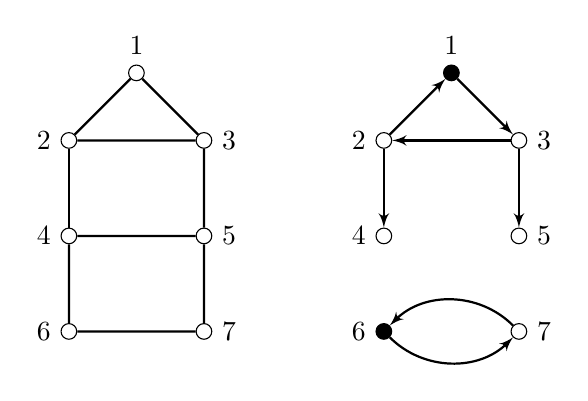
\begin{tikzpicture}
[node distance=1cm,
vertex/.style={shape=circle,draw=black,inner sep=2pt},
myedge/.style={thick},
dedge/.style={>=latex', shorten >=.0pt, shorten <=.0pt, thick}]

\node (v11) [vertex,label=above:$1$] at (0,0) {};
\node (v21) [vertex,below left=of v11,label=left:$2$] {};
\node (v31) [vertex,below right=of v11,label=right:$3$] {};
\node (v41) [vertex,below=of v21,label=left:$4$] {};
\node (v51) [vertex,below=of v31,label=right:$5$] {};
\node (v61) [vertex,below=of v41,label=left:$6$] {};
\node (v71) [vertex,below=of v51,label=right:$7$] {};
\draw[myedge] (v11) -- (v21) -- (v31) -- (v51) -- (v41) -- (v61) -- (v71)
-- (v51);
\draw[myedge] (v11) -- (v31);
\draw[myedge] (v21) -- (v41);

\node (v12) [vertex,label=above:$1$,fill] at (4,0) {};
\node (v22) [vertex,below left=of v12,label=left:$2$] {};
\node (v32) [vertex,below right=of v12,label=right:$3$] {};
\node (v42) [vertex,below=of v22,label=left:$4$] {};
\node (v52) [vertex,below=of v32,label=right:$5$] {};
\node (v62) [vertex,below=of v42,label=left:$6$,fill] {};
\node (v72) [vertex,below=of v52,label=right:$7$] {};
\draw[dedge,<-] (v12) -- (v22);
\draw[dedge,<-] (v32) -- (v12);
\draw[dedge,<-] (v22) -- (v32);
\draw[dedge,<-] (v42) -- (v22);
\draw[dedge,<-] (v52) -- (v32);

\draw[dedge,<-] (v62) [out=45,in=135] to (v72);
\draw[dedge,->] (v62) [out=-45,in=-135] to (v72);

\end{tikzpicture}
{}
\end{document}
